\section{Macchina di Turing}
La \textbf{macchina di Turing} si offre come uno dei primi
modelli per descrivere la realtà.

La realtà di cui parliamo può essere un sottoinsieme della
realtà effettiva che però deve poter essere descritta in
termini matematici.

\begin{definition}
	Una macchina di Turing (MdT) è una
	quadrupla di questo tipo
	\[
		M = \begin{pmatrix}
			Q, & \Sigma, & \delta, & q_0
		\end{pmatrix}
	\]
	dove
	\begin{itemize}
		\item $Q$ è l'insieme \emph{finito} degli stati in
		      cui si può trovare la macchina. Tra gli stati
		      abbiamo uno stato speciale $h$, con cui
		      indicheremo la corretta terminazione di un
		      calcolo $M$.
		\item $\Sigma = \{ \sigma, \sigma', \dots \}$ è
		      l'insieme \emph{finito} dei simboli, ossia,
		      l'\textbf{alfabeto} utilizzato per esprimere
		      i calcoli. Tra i simboli, abbiamo
		      \begin{itemize}
			      \item $\#$ indica il \textbf{bianco}.
			      \item $\triangleright$ è detto
			            \textbf{respingente} ed è la
			            \emph{marca} di inizio stringa.
			      \item $L$, $R$ e $-$ che non appartengono a
			            $\Sigma$ e indicano rispettivamente
			            le \emph{mosse}: \emph{Left},
			            \emph{Right} e \emph{None}.
		      \end{itemize}
		\item $q_0 \in Q$ è lo stato iniziale in cui si
		      trova la macchina.
		\item $\delta$ è la \textbf{funzione di transizione}
		      dello stato
		      \[
			      \delta \subseteq (Q \times \Sigma) \to
			      (Q \cup \{ h \}) \times \Sigma \times
			      \{ L, R, - \}
		      \]
		      che ci permette per l'appunto di cambiare lo
		      stato della macchina e progredire nel calcolo.
	\end{itemize}
\end{definition}

Arrivati a questo punto non si capisce già più niente,
cerchiamo quindi di fare ordine. L'idea è quella di
implementareLa una macchina con
\begin{itemize}
	\item Un certo numero di stati in cui trovarsi.
	\item Un certo numero di simboli che è in grado di
	      interpretare.
	\item Delle \emph{mosse} che può fare in base allo
	      stato e al simbolo correnti.
\end{itemize}
Ecco che la funzione $\delta$ diventa necessaria a far
progredire il calcolo. Come possiamo vedere dalla definizione
che ne abbiamo dato, questa prende in input una coppia di
valori. Il primo valore è uno stato, ossia lo stato
\textbf{corrente} della macchina. Il secondo valore è un
simbolo dell'alfabeto che andrà ad identificare un qualcosa
del nostro algoritmo che per ora facciamo rimanere vago.

Notiamo inoltre che la funzione $\delta$ prende in input una
coppia di valori ma ritorna una tripla composta da uno stato
$q$, che può essere anche $h$ in caso il calcolo sia terminato
con successo, un simbolo $\sigma$ e una tra le 3 mosse $L$,
$R$ e $-$.

Come vedremo, possiamo immaginare i nostri simboli disposti
su un \textbf{nastro} di lunghezza infinita, sul quale è
possibile rimanere fermi, oppure muoversi verso sinistra o
verso destra.

Ad ogni passo del calcolo, $\delta$ elabora la coppia in input
e restituisce una tripla contente il nuovo stato, il nuovo
simbolo da scrivere alla posizione attuale e come ci si deve
muovere al passo successivo.

Qualcuno potrebbe associare la MdT ad un automa a stati finiti
ma questo è in generale sbagliato perché, come vedremo, anche
se condividono alcune caratteristiche la MdT è più potente in
quanto non ha le stesse limitazioni di un automa.

Ora che abbiamo le idee più chiare, facciamo qualche
considerazione in più su $\delta$. Essa è \textbf{iniettiva},
vale cioè che, prese due triple $(q', \sigma', D')$ e
$(q'', \sigma'', D'')$ tali che
\begin{gather*}
	\delta (q, \sigma) =  (q', \sigma', D') \\
	\delta (q, \sigma) = (q'', \sigma'', D'')
\end{gather*}
allora $q' = q''$, $\sigma' = \sigma''$ e $D' = D''$.
Questo ci dice sostanzialmente che, dato uno stato e un simbolo
c'è un solo altro stato in cui possiamo andare. Un'altra cosa
da specificare è che per $\delta$ vale sempre che se
\[ \delta(q, \start) = (q', \sigma, D) \]
allora $\sigma = \start$ e $D = R$. Questo ci dice
sostanzialmente che se ci troviamo all'inizio del nastro
possiamo andare solo a destra.

Dato che $Q$ e $\Sigma$ sono insiemi finiti, anche gli elementi
di $\delta$ sono finiti e dunque che, come ricordiamo sono le
condizioni necessarie descritte nell'idea intuitiva di
algoritmo.


\subsection{Alfabeto}
I dati su cui opera una MdT sono stringhe $w$ di caratteri
appartenenti a $\Sigma$, più precisamente $w \in \Sigma^*$,
dove $\Sigma^*$ comprende anche la stringa vuota $\epsilon$.

Senza stare a incasinarsi con inutili formalismi matematici,
se $\Sigma$ è l'alfabeto, allora $\Sigma^*$ è l'insieme di
tutte le possibili stringhe generabili con quell'alfabeto e
la stringa vuota.

\begin{example}
	Prendiamo ad esempio l'alfabeto binario
	\begin{gather*}
		\Sigma = \{ 0, 1 \} \\
		\Downarrow \\
		\Sigma^* = \{ \epsilon, 0, 1, 01, 10, 11, \dots \}
	\end{gather*}
\end{example}

\subsection{Computazione}
Iniziamo ora a vedere come opera una MdT su qualche problema
di esempio. La \textbf{configurazione corrente} di una MdT
viene identificata $(q, u, \sigma, v)$ dove
\begin{itemize}
	\item $q$ è lo stato corrente.
	\item $u$ è la stringa a sinistra del carattere attuale.
	\item $\sigma$ è il carattere attuale.
	\item $v$ è il resto della stringa che termina con un
	      carattere non nullo.
\end{itemize}
La situazione corrente di una MdT può essere espressa più
comodamente con $(q, u \underline{\sigma} v)$. Graficamente
una MdT appare in questo modo
\begin{center}
	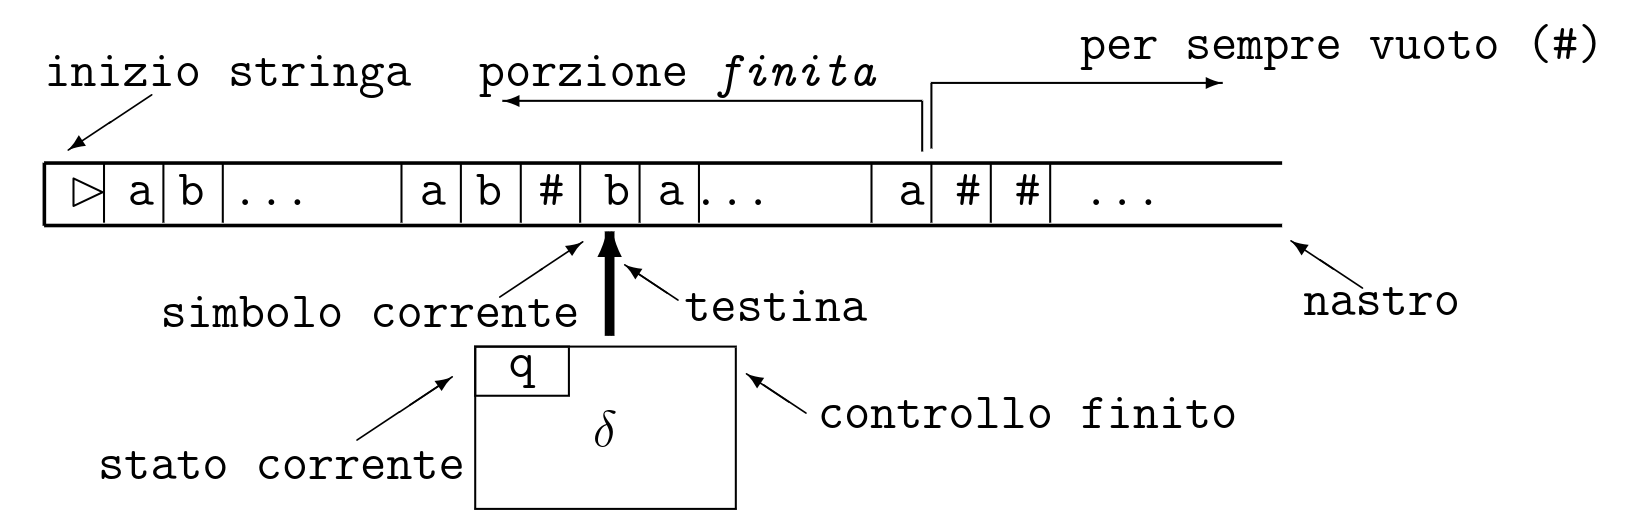
\includegraphics[scale=0.225]{images/turing.png}
\end{center}
Tenendo a mente questa figura possiamo provare a fare il primo
esempio di calcolo eseguito da una MdT.

\begin{example}
	Iniziamo con il fare l'esempio di una MdT i cui stati
	possibili sono due $Q = \{ q_0, q_1 \}$ e il cui alfabeto
	è composto come segue $\Sigma = \{ \#, \start, a \}$.
	La funzione $\delta$ di transizione è invece rappresentata
	dalla seguente tabella.
	\begin{center}
		\begin{tabular}{| c | c | c |}
			\hline
			$q$   & $\sigma$ & $\delta(q, \sigma)$ \\
			\hline
			$q_0$ & $\start$ & $q_0, \start, R$    \\
			$q_0$ & $\#$     & $h, \#, -$          \\
			$q_0$ & $a$      & $q_1, \#, L$        \\
			$q_1$ & $\#$     & $q_0, \#, L$        \\
			$q_1$ & $a$      & $q_0, a, -$         \\
			\hline
		\end{tabular}
	\end{center}
	A questo punto cerchiamo di capire cosa fa questa MdT
	quando si introduce una stringa (valida) in input.
	Come \textbf{configurazione} iniziale prendiamo
	\[ q_0/ \start \# \# a \# a \underline{a} \# \]
	dove $\underline{a}$ indica che il \textbf{cursore} è
	posizionato su quel carattere. La tabella ci dice che
	\[ \delta (q_0, a) = q_1, \#, L \]
	questo significa che dobbiamo passare allo stato $q_1$,
	rimpiazzare $a$ con $\#$ e muovere il cursore a sinistra.
	La nuova configurazione sarà quindi
	\[ q_1/ \start \# \# a \# \underline{a} \# \# \]
	A questo punto, seguendo la tabella, i restanti passaggi
	seguono tutti la solita progressione.
	\begin{gather*}
		q_1/ \start \# \# a \# \underline{a} \# \# \\
		q_0/ \start \# \# a \# \underline{a} \# \# \\
		q_1/ \start \# \# a \underline{\#} \# \# \# \\
		q_1/ \start \# \# \underline{a} \# \# \# \# \\
		q_0/ \start \# \# \underline{a} \# \# \# \# \\
		q_1/ \start \# \underline{\#} \# \# \# \# \# \\
		q_0/ \start \underline{\#} \# \# \# \# \# \# \\
		h/ \start \underline{\#} \# \# \# \# \# \#
	\end{gather*}
	Come possiamo vedere il calcolo è terminato con successo
	e questa macchina aveva lo scopo di cancellare ogni
	carattere della stringa iniziale.
\end{example}
Per vedere una MdT in azione è possibile visitare questo
\href{https://turingmachinesimulator.com/}{sito} in cui è
possibile programmare una MdT oppure eseguire esempi già
proposti.

\subsubsection{Configurazione e computazione}
Come abbiamo detto precedentemente, una \textbf{configurazione}
è definita dalla quadrupla
\[ \gamma = (q, u, \sigma, v) \]
Ciò che non abbiamo detto è che gli elementi di $\gamma$
appartengono al seguente insieme
\[
	\gamma \in (Q \cup \{ h \}) \times
	\Sigma^* \times \Sigma \times \Sigma^F
\]
L'ultimo insieme ($\Sigma^F$) è un po' particolare, infatti
tale insieme è definito come
\[
	\Sigma^F = \Sigma^* \cdot \left( \Sigma \backslash
	\{ \# \} \right) \cup \{ \epsilon \}
\]
quindi possiamo scrivere la stringa $v$ come
$\sigma_0 \sigma_1 \dots \sigma_n$, con $\sigma_n \neq \#$,
al posto della stringa infinita composta dai vari $\sigma$ e
con infiniti $\#$ alla fine.

Si noti però che un qualsiasi carattere $\sigma_i$ con $i < n$
può essere $\#$ ed inoltre la stringa $u$ può essere vuota
solo quando il carattere corrente è $\start$. La convenzione
impone quindi di scrivere la configurazione iniziale del primo
esempio fatto, in questo modo
\[ (q_0, \start \# \# a \# a, a, \epsilon) \]

\begin{definition}
	Una \textbf{computazione} è una successione finita di
	passi
	\[ (q_0, w) \to^* (q', w') \]
	dove $\to^*$ è la chiusura riflessiva e transitiva di
	$\to$. Ovviamente se vi sono $n$ passi, la computazione
	è lunga $n$ e dunque scriveremo $\to^n$.
\end{definition}

Definiamo meglio cos'è un \textbf{passo di computazione}.
Proviamo a definire un passo di computazione per casi,
considerando $a, b, c$ elementi generici di $\Sigma$.
\begin{itemize}
	\item $(q, u \underline{a} v) \to (q', u \underline{b} v)$
	      se $\delta (q, a) = (q', b, -)$.
	\item $(q, u c \underline{a} v) \to
		      (q', u \underline{c} b v)$
	      se $\delta (q, a) = (q', b, L)$.
	\item \begin{enumerate}
		      \item $(q, u \underline{a} c v) \to
			            (q', u b \underline{c} v)$
		            se $\delta (q, a) = (q', b, R)$.
		      \item $(q, u \underline{a}) \to
			            (q', u b \underline{\#})$
		            se $\delta (q, a) = (q', b, R)$.
	      \end{enumerate}
\end{itemize}
In questo modo garantiamo che ciascun passo abbia effetto
limitato sulle configurazioni, come richiesto dalla seconda
parte del punto 2 nell'idea intuitiva dell'algoritmo.

Allo stesso modo possiamo immaginarci che se partiamo da uno
stato iniziale $(q_0, \underline{\start} w)$, dopo un certo
numero di passi arriviamo in uno stato $(q', w')$.

\begin{definition}
	Diciamo che una computazione \textbf{termina} o
	\textbf{converge} ($\downarrow$) se e solo se lo stato
	finale è $h$. Nell'esempio fatto qui sopra $q' = h$.

	Diciamo invece che la computazione \textbf{non termina}
	o \textbf{diverge} ($\uparrow$) se e solo se per ogni
	$q'$ e $w'$ tali che
	\[ (q_0, w) \to^* (q', w') \]
	esistono $q''$ e $w''$ tali che
	\[ (q', w') \to^* (q'', w'') \]
	ovvero tali che si continua sempre a fare un passo.
\end{definition}

Come possiamo vedere, le MdT definite in questo modo,
rispettano l'idea intuitiva di algoritmo che abbiamo dato
all'inizio.

\begin{example}
	Facciamo un esempio di computazione che non termina mai
	tramite una macchine che semplicemente non contiene il
	simbolo $h$ di terminazione.
	\begin{center}
		\begin{tabular}{|c|c|c|}
			\hline
			$q$   & $\sigma$ & $\delta$             \\
			\hline
			$q_0$ & $\start$ & $q_0$, $\start$, $R$ \\
			$q_0$ & $a$      & $q_0$, $a$, $R$      \\
			$q_0$ & $\#$     & $q_0$, $\#$, $R$     \\
			\hline
		\end{tabular}
	\end{center}
\end{example}

Proviamo ora a fare un esempio più concreto di una MdT che
calcola qualcosa di più sensato rispetto agli esempi visti
fino ad ora.

\begin{example}
	Questa MdT si propone di calcolare la somma di due numeri
	$n$ ed $m$, dove $n$ ed $m$ sono rappresentati in notazione
	unaria tramite il simbolo $|$ ripetuto $n$ (o $m$) volte.
	La funzione $\delta$ è definita dalla seguente tabella
	\begin{center}
		\begin{tabular}{|c|c|c|}
			\hline
			$q$   & $\sigma$ & $\delta$         \\
			\hline
			$q_0$ & $\start$ & $q_0, \start, R$ \\
			$q_0$ & $|$      & $q_0, |, R$      \\
			$q_0$ & $+$      & $q_1, |, R$      \\
			$q_1$ & $|$      & $q_1, |, R$      \\
			$q_1$ & $\#$     & $q_2, \#, L$     \\
			$q_2$ & $|$      & $h, \#, -$       \\
			\hline
		\end{tabular}
	\end{center}
	Il simbolo $+$ deve essere tra le due sequenze di $|$.
	Proviamo ora ad eseguire la computazione per il calcolo
	di $1 + 2$, partendo dalla configurazione iniziale
	\[ q_0/ \quad \underline{|} + | | \]
	Svolgiamo quindi i seguenti passi
	\begin{gather*}
		(q_0, \; \underline{\start} | + | | ) \to
		(q_0, \; \start \underline{|} + | | ) \\
		(q_0, \; \start \underline{|} + | | ) \to
		(q_0, \; \start | \underline{+} | | ) \\
		(q_0, \; \start | \underline{+} | | ) \to
		(q_1, \; \start | | \underline{|} | ) \\
		(q_1, \; \start | | \underline{|} | ) \to
		(q_1, \; \start | | | \underline{|} ) \\
		(q_1, \; \start | | | \underline{|} ) \to
		(q_1, \; \start | | | | \underline{\#} ) \\
		(q_1, \; \start | | | | \underline{\#} ) \to
		(q_2, \; \start | | | \underline{|} \# ) \\
		(q_2, \; \start | | | \underline{|} \# ) \to
		(h, \; \start | | | \underline{\#} \# )
	\end{gather*}
	per concludere che il calcolo termina dato che siamo
	giunti nello stato speciale $h$. Come possiamo vedere il
	nostro risultato è dato dal numero di $|$ rimanente.
\end{example}

Un altro tipico esempio di utilizzo di queste macchine è
quello di decidere se una stringa è palindroma. In questo
caso descriviamo brevemente quale sarebbe l'idea.
\begin{enumerate}
	\item Si controlla il primo carattere della stringa, lo si
	      sovrascrive con $\start$ e si passa in uno stato
	      specifico per quel carattere (supponendo che il primo
	      carattere sia $a$, si passa in $q_a$).
	\item Si arriva in fondo alla stringa e si controlla che
	      l'ultimo carattere sia uguale al primo, se sì, lo
	      si sovrascrive con un $\#$.
	\item Si torna indietro fino al primo $\start$ che si
	      incontra.
\end{enumerate}
Si ripete il procedimento finché non si esaurisce tutta la
stringa o finché non fallisce.

